\chapter{Application of the Approach}
\label{ch:SolutionApplication}
This chapter applies the previously presented approach to identify microservices from the business point of view, using clustering on control flow and data flow. It is applied to CoCoME, whose system specifications are defined in chapter \ref{ch:CoCoME}. Speaking of the order, this chapter follows the process overview illustrated by Fig.\ref{fig:thesisProcess}.

\section{Use Cases as BPMN Models}
\label{sec:SolutionApplication:TransformUseCases}
CoCoME's system specifications are given in terms of use cases. A short overview is available in chapter \ref{ch:CoCoME}, whereas a more detailed version can be found in the \textit{Technical Report} \cite{CoCoMETechnical}. We decide to omit  \textit{UC 8 - Product Exchange} as independent BPMN model, because both reference sets either did not take it into consideration or implemented it differently. However, it was added as extension to \textit{UC 1} as single activity named \textit{Product Exchange}. In the same way, \textit{UC 2 - Manage Express Checkout} is added to \textit{UC 1} as single activity named \textit{Manage Express Checkout}. \textit{UC 2} extends \textit{UC 1} and therefore, has to be associated with \textit{UC 1} anyway.  Fig.\ref{fig:UC1} illustrates \textit{UC 1,2} and \textit{8} as BPMN model. The remaining BPMN models are available in the appendix (cf. \ref{sec:appendix:BPMN Models}). For the sake of clarity, the models are not yet joined as described in section \ref{sec:PrepApproach:TransformUCtoBPMN}. Apart from Fig.\ref{fig:UC1}, each use case is illustrated as single BPMN process. However, the BPMN models that represent \textit{UC 3} and \textit{UC 4} as well as \textit{UC 4} and \textit{UC 1} need to be joined, as preconditions and postconditions are equal. 




%"l, b, r, t"
\begin{figure}[h!]
	\centering
	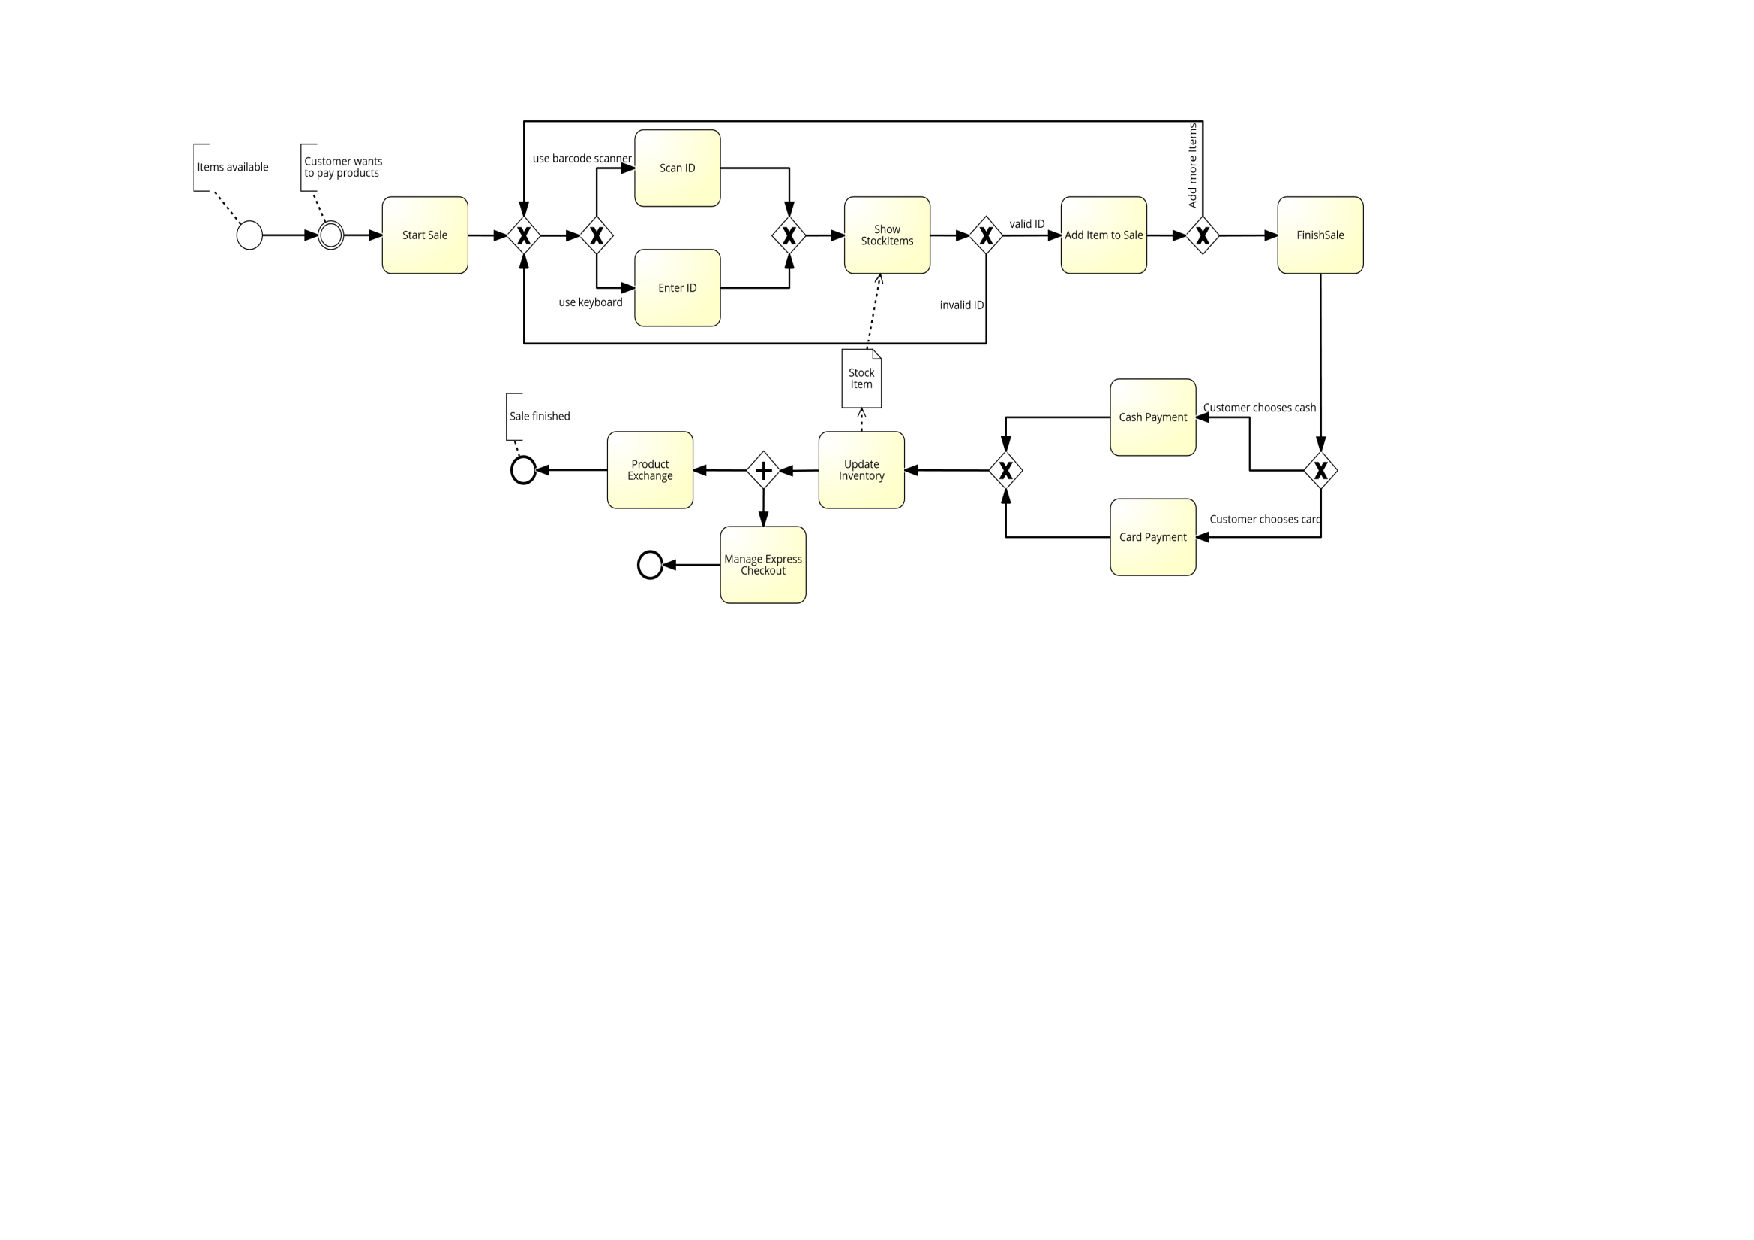
\includegraphics[width=\textwidth, trim={4cm 10.9cm 8cm 2.3cm}]{img/UC1.pdf}
	\caption{UC1 - Process Sale (with UC2 and UC8)}
	\label{fig:UC1}
\end{figure}

\FloatBarrier


\section{Extracted Control Flow}
\label{sec:SolutionApplication:ExtractDataFlow}
In this step, the control flow is extracted from the BPMN models. Sec. \ref{sec:Solution:ExtractControlFlow} provides the detailed extraction process, but in a word, everything but the control flow elements are deleted. Fig.\ref{fig:UC3Control} presents the control flow for \textit{UC 3}. The remaining control flow diagrams are available in the appendix (cf. \ref{sec:appendix:ControlFlow}).  

%"l, b, r, t"
\begin{figure}[h!]
	\centering
	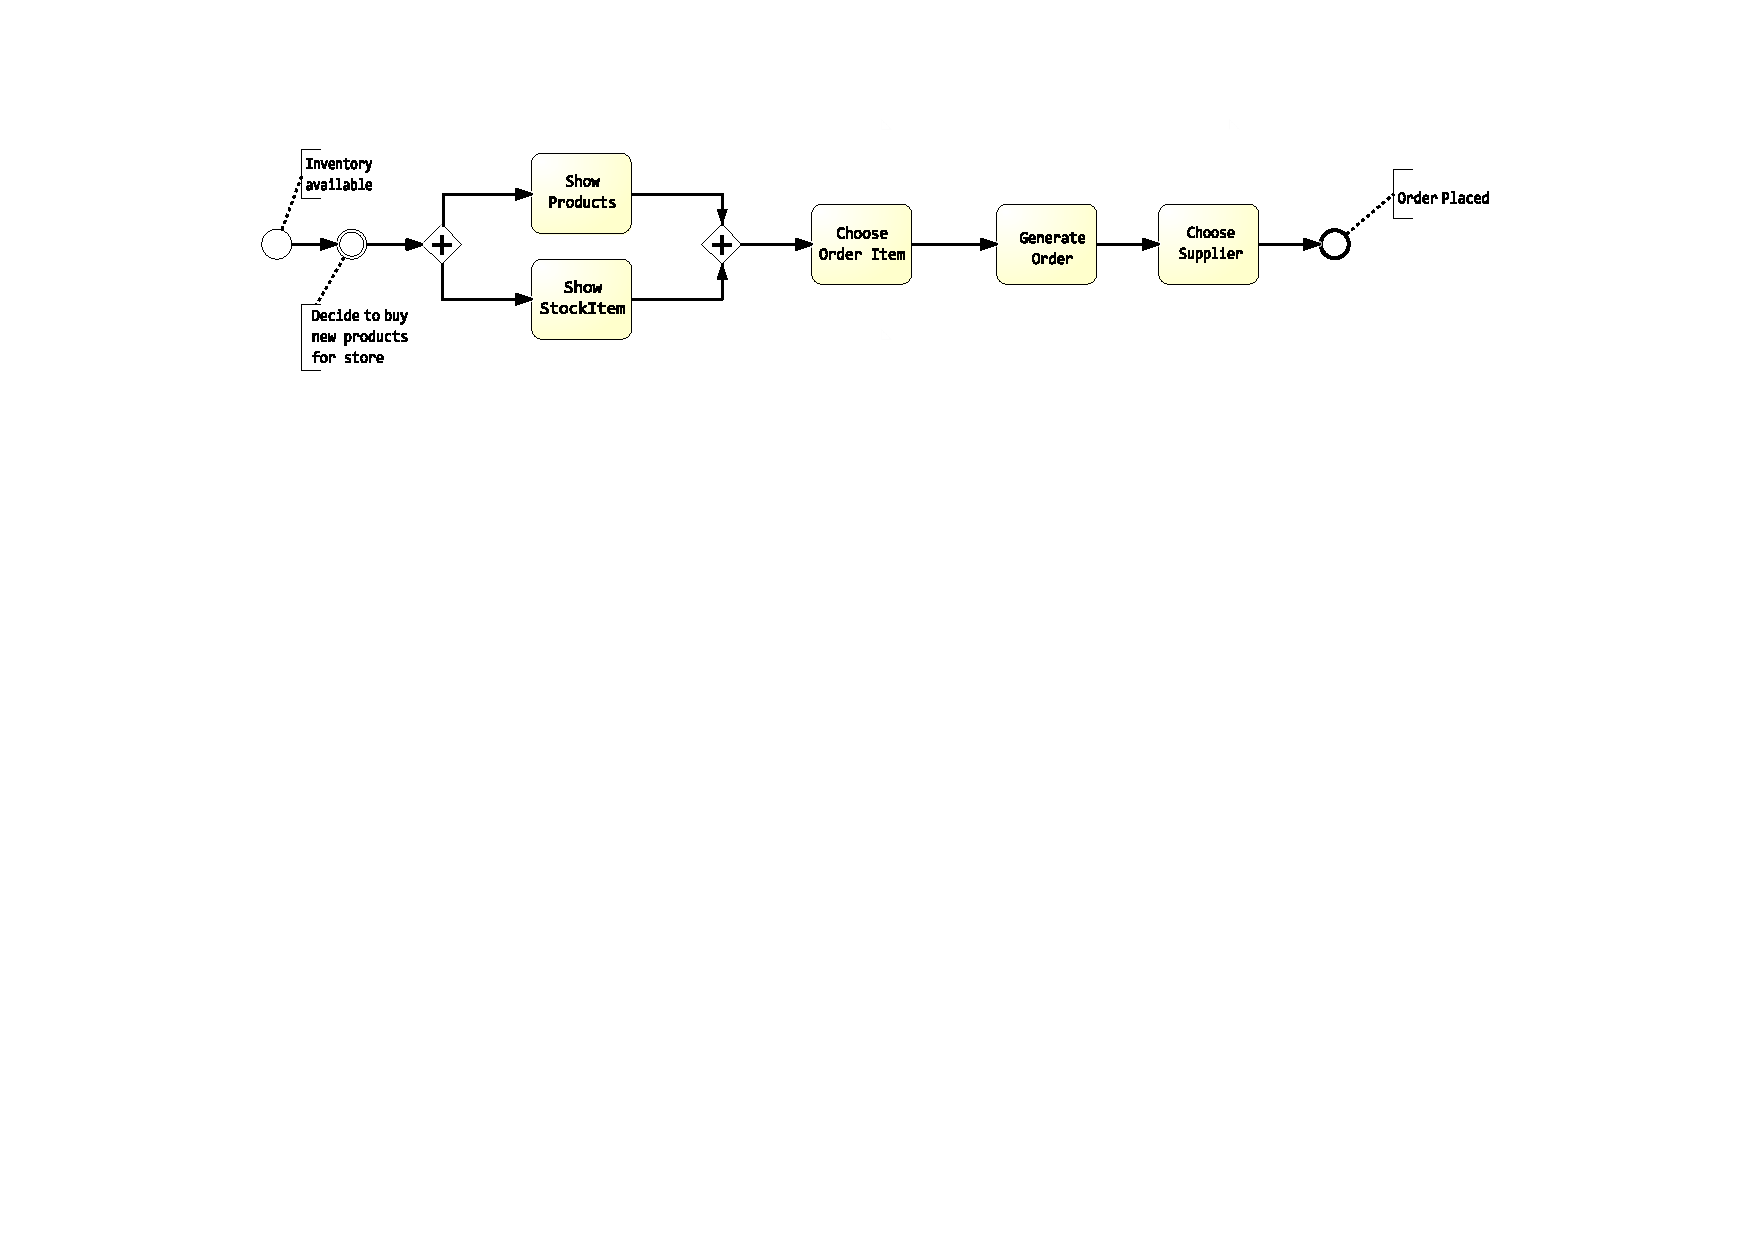
\includegraphics[width=\textwidth, trim={5cm 14.5cm 6cm 2.5cm}]{img/UC3Control.pdf}
	\caption{Control Flow UC3 - Order Products}
	\label{fig:UC3Control}
\end{figure}

\section{Extracted Data Flow}
\label{sec:SolutionApplication:ExtractControlFlow}
Like the previous step, the data flow is extracted from the BPMN models as described in Sec.\ref{sec:Solution:ExtractDataFlow}. Fig.\ref{fig:UC3Control} presents the data flow for \textit{UC 3}. The remaining data flow diagrams are available in the appendix (cf. \ref{sec:appendix:DataFlow}).

%"l, b, r, t"
\begin{figure}[h!]
	\centering
	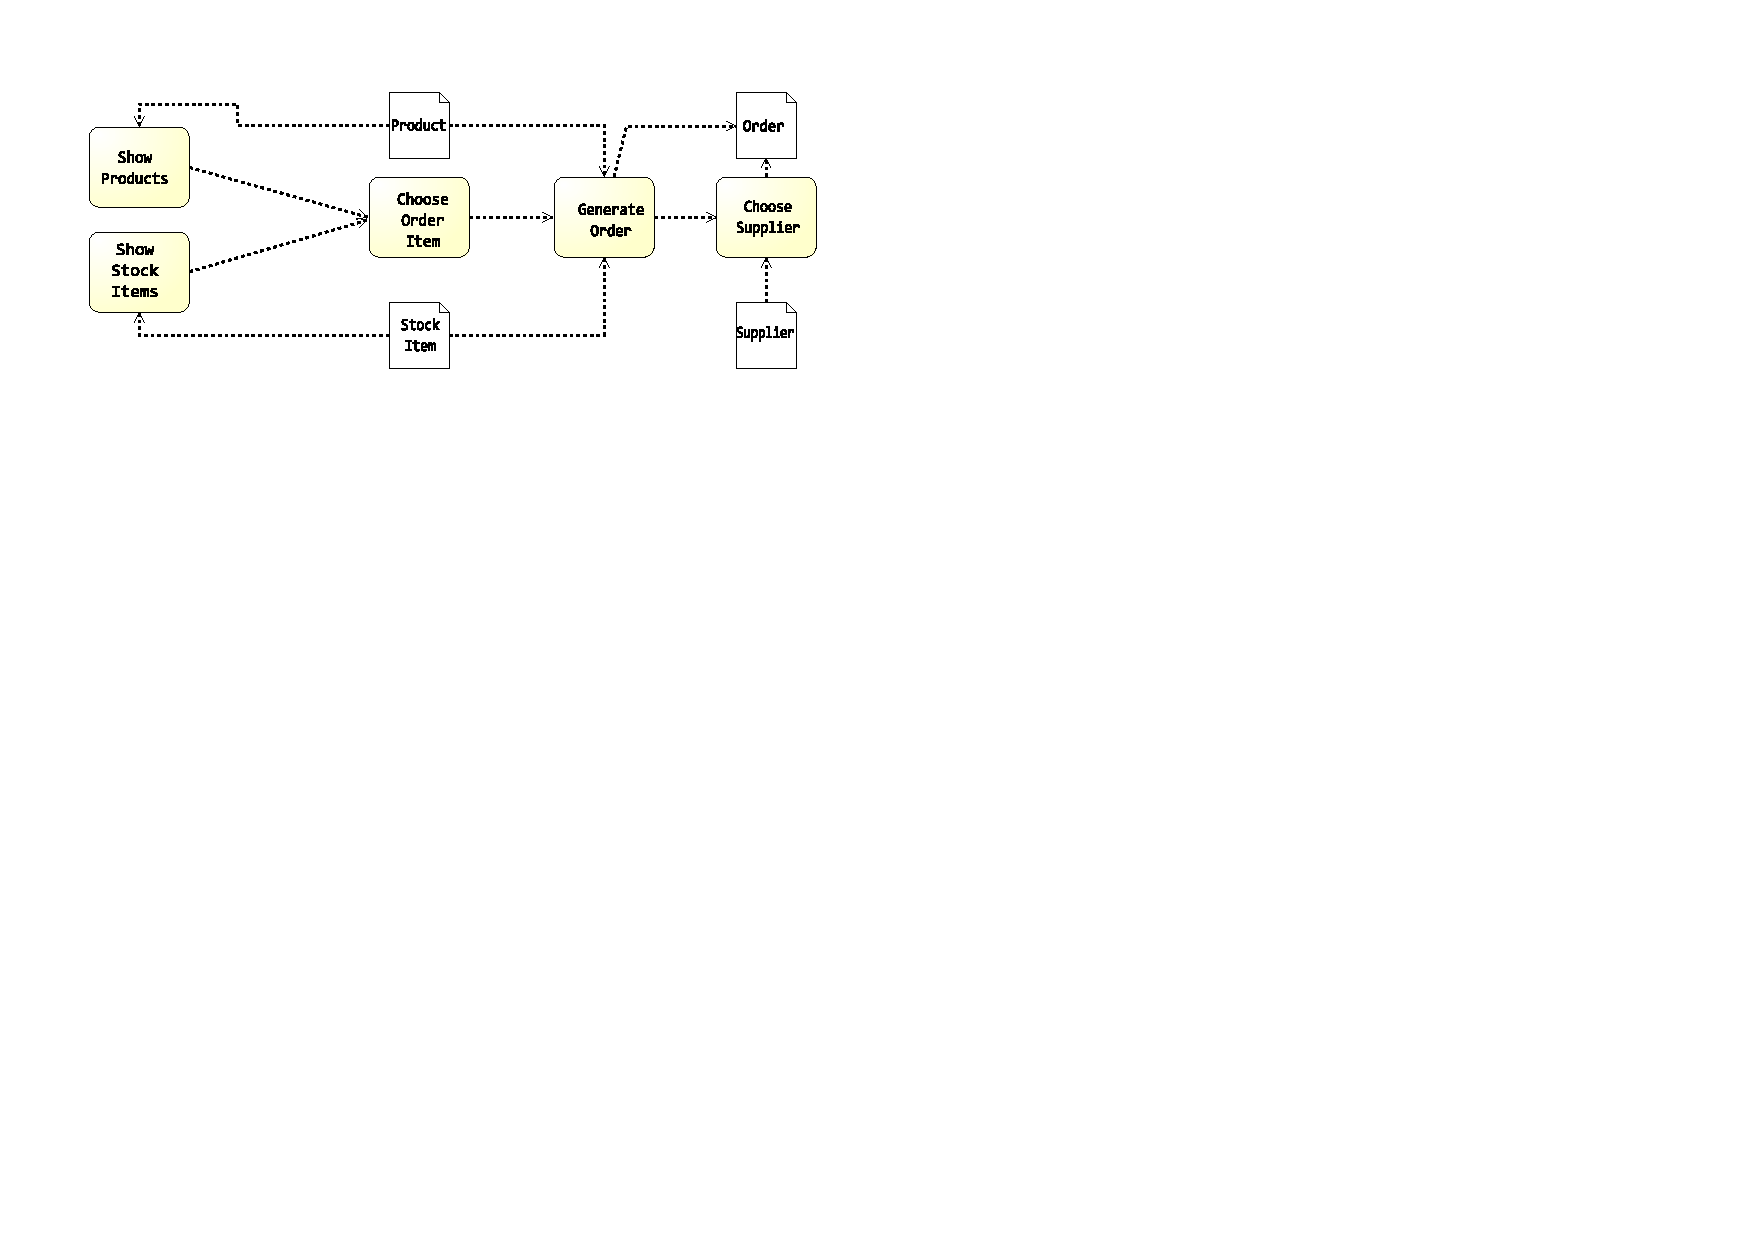
\includegraphics[width=8cm, trim={5cm 14cm 17cm 0cm}]{img/UC3DFD.pdf}
	\caption{Control Flow UC3 - Order Products}
	\label{fig:UC3DFD}
\end{figure}

\section{Control Flow Graph}
\label{sec:SolutionApplication:ControlFLowGraph}
Fig.\ref{fig:CoCoMEControlFlowGraph} illustrates the control flow graph of CoCoME which is derived from the control flow diagrams. 

%"l, b, r, t"
\begin{figure}[h!]
	\centering
	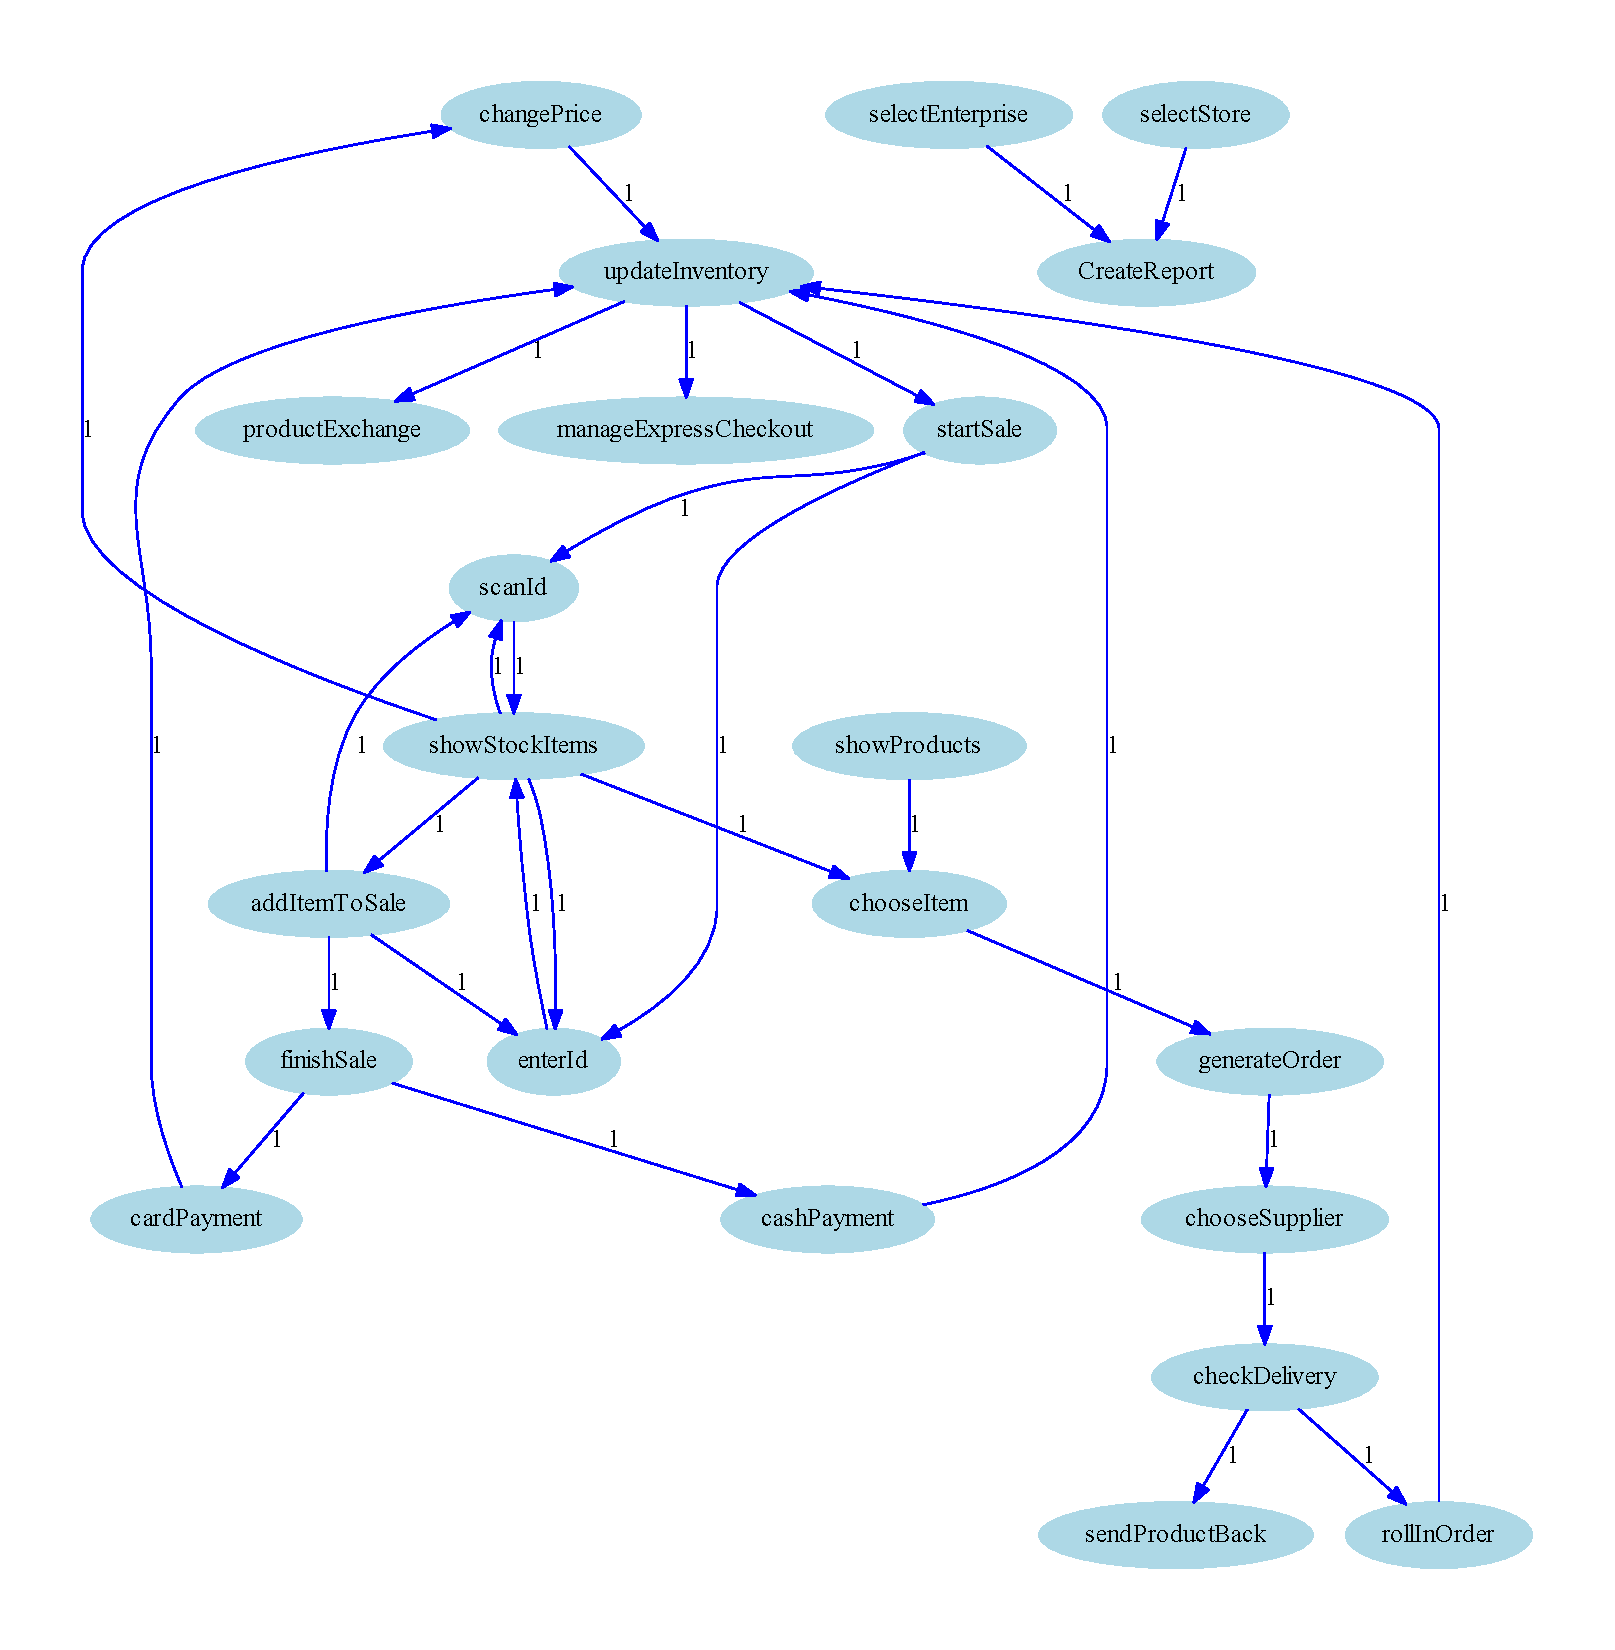
\includegraphics[width=\textwidth, trim={2cm 0cm 2cm 0cm}]{img/CoCoMEControlFlowGraph.pdf}
	\caption{Control Flow Information as Graph CoCoME}
	\label{fig:CoCoMEControlFlowGraph}
\end{figure}


\section{Data Flow Graph}
\label{sec:SolutionApplication:DataFLowGraph}
Fig.\ref{fig:CoCoMEDataFlowGraph} illustrates the data flow graph of CoCoME which is derived from the data flow diagrams. When identifying the data flow dependencies, it is necessary to choose a value for the parameter \textit{n}, that describes the maximum distance between a pair of activities that consume and produce a data object. We use \textit{n=1}, as it produces the most appropriate results compared to the final microservice decomposition. 

%"l, b, r, t"
\begin{figure}[h!]
	\centering
	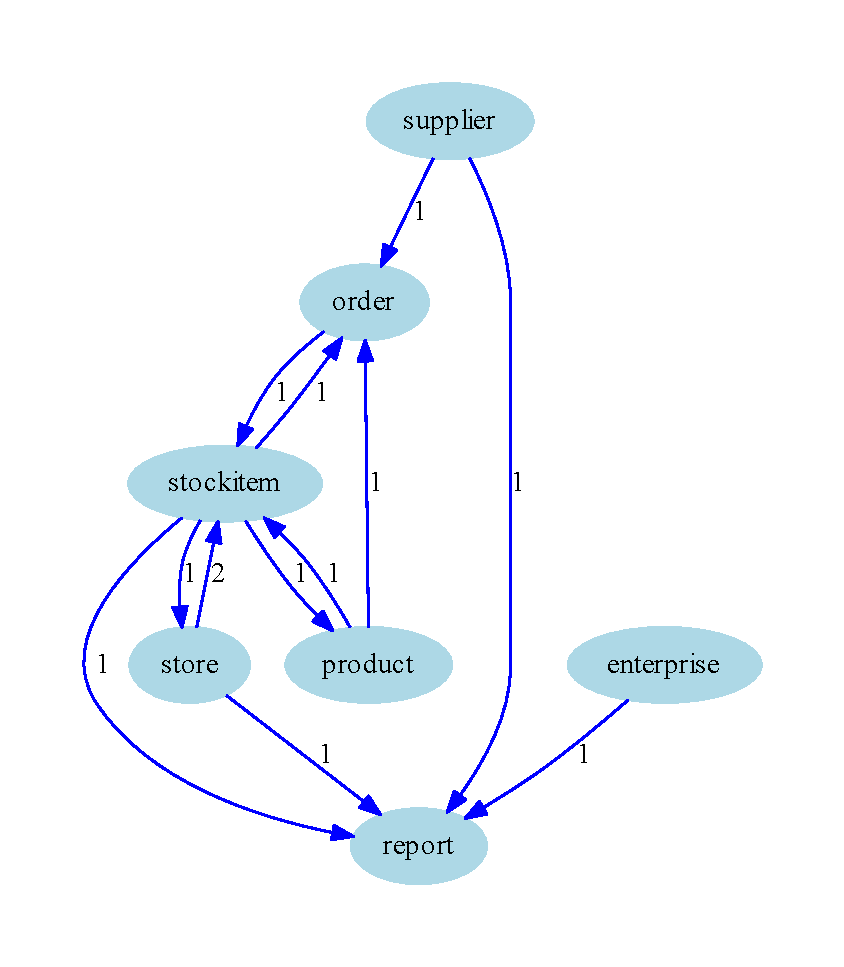
\includegraphics[width=10cm, trim={1cm 0cm 2cm 0cm}]{img/CoCoMEDataFlowGraph.pdf}
	\caption{Data Flow Information as Graph CoCoME}
	\label{fig:CoCoMEDataFlowGraph}
\end{figure}

\pagebreak

\section{Activity Clusters}
\label{sec:SolutionApplication:ActivityCluster}
Fig.\ref{fig:CoCoMEActivityCluster} shows the activity clusters that are identified using the clustering algorithm described in Sec.\ref{sec:Solution:IdentifyCluster}. The naming is inspired by the implementation of CoCoME \cite{NikoCoCoMEImpl}.

%"l, b, r, t"
\begin{figure}[h!]
	\centering
	\begin{sideways}
		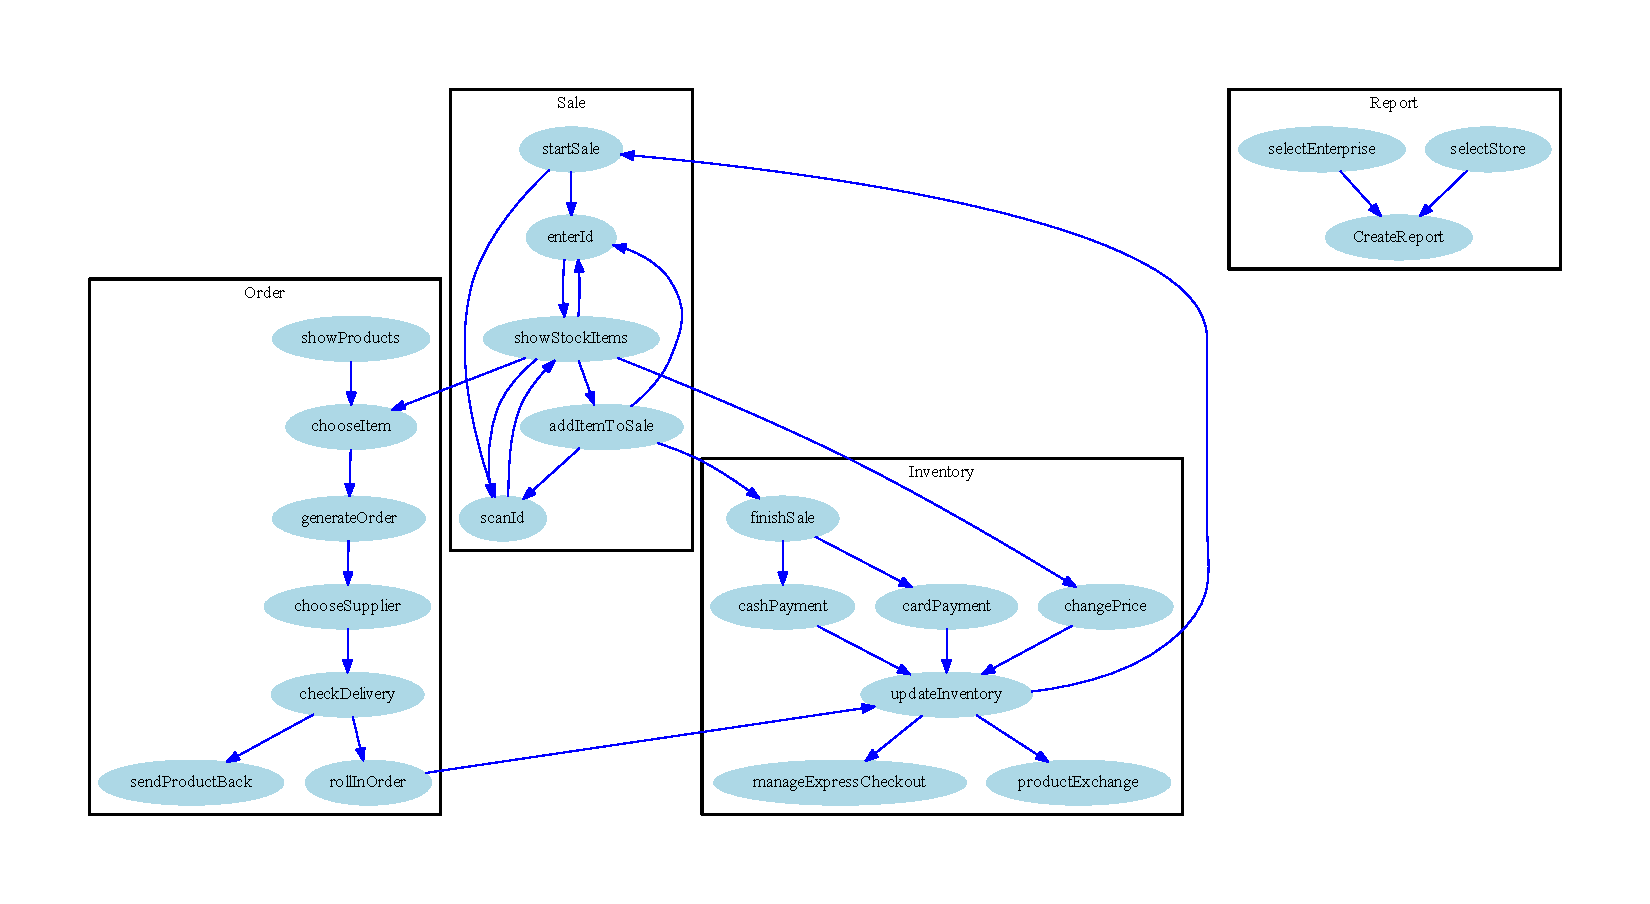
\includegraphics[width=19.0cm, trim={1.5cm 0cm 1.8cm 0cm}]{img/CoCoMEActivityCluster.pdf}
	\end{sideways}
	
	\caption{Clustering on CoCoME's Activities}
	\label{fig:CoCoMEActivityCluster}
\end{figure}

\FloatBarrier

\section{Data Object Clusters}
\label{sec:SolutionApplication:DataObjectCluster}
Fig.\ref{fig:CoCoMEActivityCluster} shows the data object clusters that are identified using the clustering algorithm described in Sec.\ref{sec:Solution:IdentifyCluster}.
%"l, b, r, t"
\begin{figure}[h!]
	\centering
	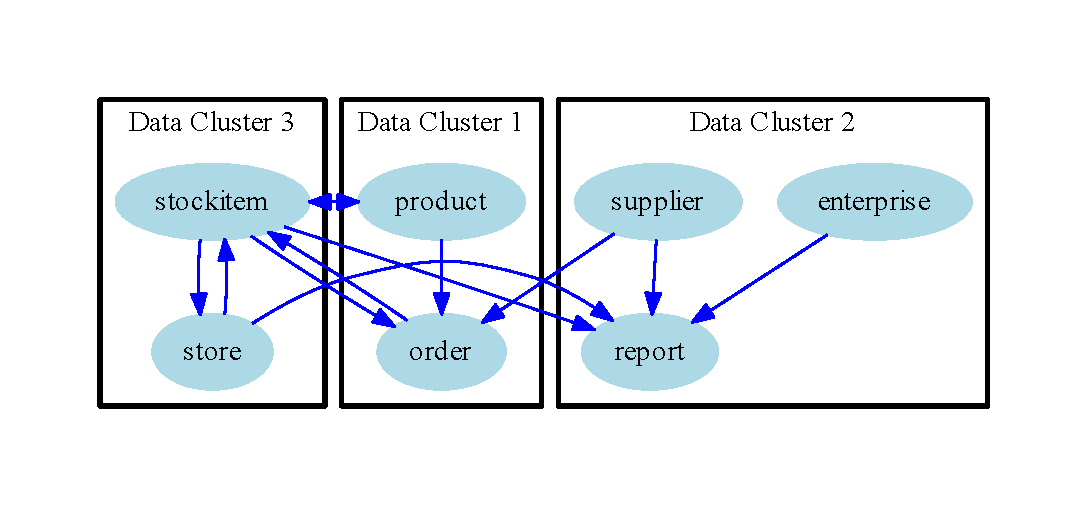
\includegraphics[width=12cm, trim={2cm 0cm 2cm 0cm}]{img/CoCoMEDataClusterWith1.pdf}
	\caption{Clustering on CoCoME's Data Objects}
	\label{fig:CoCoMEDataCluster}
\end{figure}

\section{Match Clusters}
\label{sec:SolutionApplication:MatchCluster}
In the following, the data object clusters and the activity clusters are matched. Section \ref{sec:Solution:MatchCluster} provides several solutions, including one that is only given conceptional and still raises too many uncertainties. Consequently, the matching is done by applying the black box clustering approach. Hence, the data access dependencies between data object and activity cluster need to be elaborated first. \\




%"l, b, r, t"
\begin{figure}[h!]
	\centering
	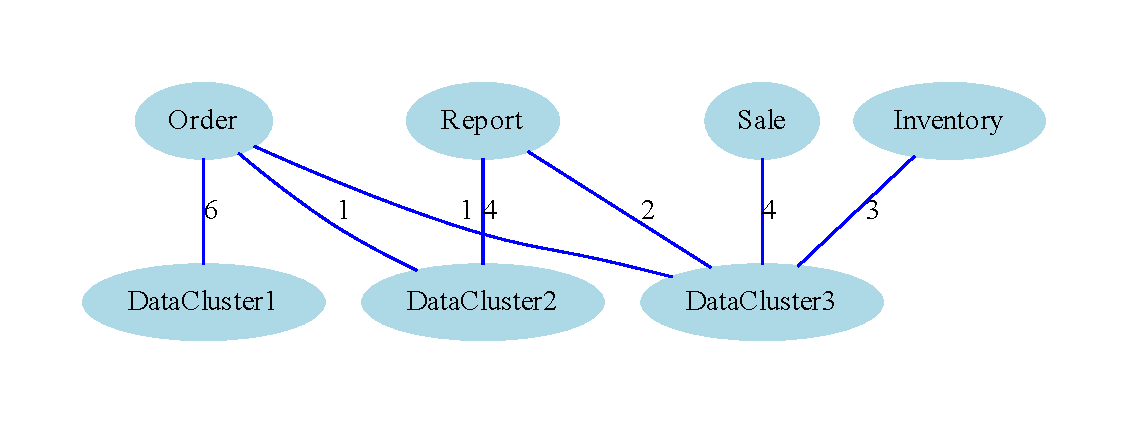
\includegraphics[width=12cm, trim={2cm 1cm 2cm 0cm}]{img/MatchClusterGraph.pdf}
	\caption{Data Access Dependencies between Data Object Clusters and Activity Cluster of CoCoME}
	\label{fig:CoCoMEClusterGraph}
\end{figure}

\noindent
Fig.\ref{fig:CoCoMEClusterGraph} illustrates the data access dependencies between the four activity clusters \textit{Order, Report, Sale} and  \textit{Inventory} and the \textit{DataClusters 1-3}. The weights correspond to the amount of read and write accesses between activities and data objects within the corresponding clusters.  \\
Finally, the clustering method introduced in Sec.\ref{sec:Solution:IdentifyCluster} identifies cohesive clusters of activity cluster nodes and data object cluster nodes.



%"l, b, r, t"
\begin{figure}[h!]
	\centering
	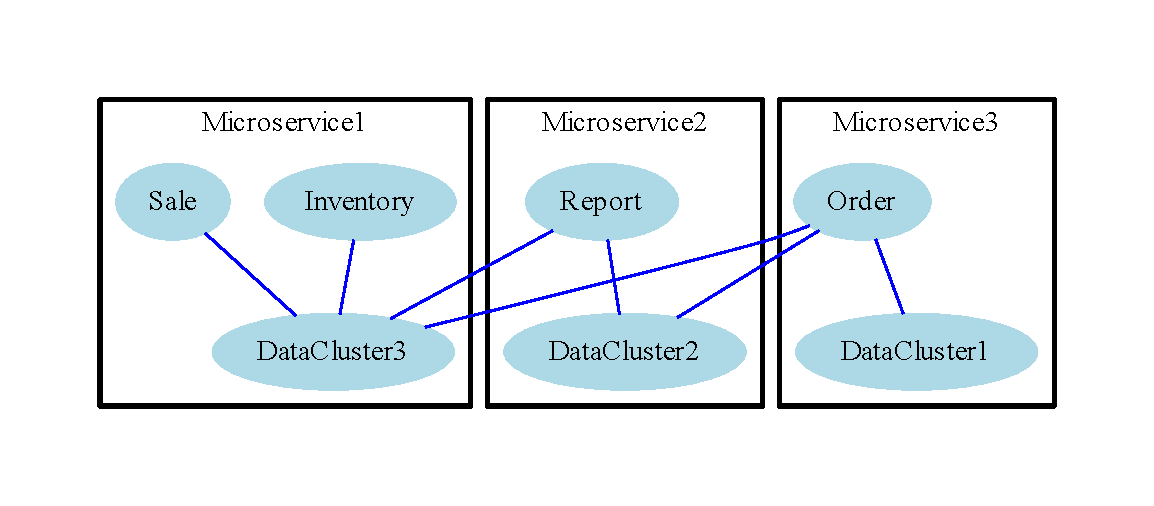
\includegraphics[width=12cm, trim={2cm 1cm 2cm 1cm}]{img/MatchClusterClustering.pdf}
	\caption{Proposed Microservice Decomposition of CoCoME}
	\label{fig:CoCoMEClusterMatching}
\end{figure}



\section{Extract Microservice Candidates}
\label{sec:SolutionApplication:ExtractMicroserviceCandidates}
In the previous step, cohesive clusters of activity cluster nodes and data object cluster nodes are identified. Each of the combined clusters correspond to a microservice candidate. Fig.\ref{fig:CoCoMEClusterMatching} illustrates the  microservices that are identified. To compare the outcome with other results, it is necessary to elaborate the functionality that is provided by each microservice as well as the accompanying data objects. To be able to compare it with the reference sets, the functionalities must be renamed and abstracted. For example, \textit{startSale} and \textit{finishSale} become \textit{Handle sale} or \textit{enterId} and \textit{showStockItems} become \textit{Identify stock items}. \\



\begin{multicols}{3}
	\textbf{Microservice 1}
	\begin{flushleft}
	\begin{itemize}[noitemsep]
	\item Handle sale
	\item Handle payment
	\item Manage express checkout
	\item Exchange products
	\item Identify stock items
	\item Handle inventory
	\item Change price
	\item \textbf{Data objects}: stockItem, store
	\end{itemize}
	\end{flushleft}


	\vfill
	\columnbreak
	\textbf{Microservice 2}
	\begin{flushleft}
	\begin{itemize}[noitemsep]
	\item Create delivery report
	\item Create stock report
	\item \textbf{Data Objects}: supplier, report, enterprise
    \item[]
    \item[]
    \item[]
    \item[]
    \item[]
	\end{itemize}
	\end{flushleft}
	
	
	\vfill
	\columnbreak
	\textbf{Microservice 3}
	\begin{flushleft}
	\begin{itemize}[noitemsep]
		\item Show products
		\item Create orders
		\item Handle deliveries
		\item Show suppliers
		\item \textbf{Data Objects}: product, order
	\end{itemize}
\end{flushleft}
\end{multicols}











